\section{Решение для линейноного осцилятора}
\subsection{Приближения и уточнение формулировки}

Во первых вспомнм что:
\begin{equation}
    p  = \cfrac{mv}{\sqrt{1 - \cfrac{v^2}{c^2}}}.
\end{equation}
В не релятивистком случае уравненнеие сильно упрощается:
\begin{equation}
    p \approx mv,
\end{equation}
поэтому предлагаю решать в приближении $v/c \ll 1$.
Тогда известное нам уравнение:
\begin{equation}
    \cfrac{dp}{dt} = e  E + \cfrac{e}{c} \insqr{ v,  H},
\end{equation}
выродится в: 
\begin{equation}
    m\cfrac{dv}{dt} = e  E.
\end{equation}
От сюда следует что можно пренебречь влиянием магнитного поля на диполь и 
рассматривать только электрическое поле. 

\subsection{Диф. уравнение}
 
Запишем наше уравнение:
\begin{equation}
    m \ddot r + mk\dot r + m\omega_0^2r = e E(t).
\end{equation}
Как уже ясно я предлагаю использовать преобразование фурье для решения:
\begin{equation}
    -\omega^2 r - i\omega kr + \omega_0^2r = \cfrac{e}{m} E_\omega.
\end{equation}
Вспомним что в излучение диполя основной вклад дает компонента $\ddot d$,
А так как так как центральный заряд не подвижен и закреплен в начале СО 
то $d = e r \implies \ddot{d} = e\ddot{{r}}$. Тогда 
нам нужно искать:
\begin{equation}
    r = \cfrac{eE_\omega}{m\inner{\omega_0^2 - i\omega k - \omega^2 }}.
\end{equation}
\begin{equation}
    \mathfrak F \insqr{\ddot d}(\omega)= -e\omega^2 r = 
    -\cfrac{e\omega^2E_\omega}{m\inner{\omega_0^2 - i\omega k 
    - \omega^2 }}.
    \label{eq:ddot_d}
\end{equation}

Получим распределение полей в общем виде, подставив $\ddot d$ в \ref{eq:2.5}:
\begin{equation}
    H = \cfrac{e}{mc^2R}\insqr{\int_\re
    \cfrac{\omega^2E_\omega}{\inner{\omega_0^2 - i\omega k - \omega^2 }}\exp{-it\omega}\cfrac{d\omega}{2\pi}, n},
    \label{eq:fild}
\end{equation}
\begin{equation}
    E = \insqr{H, n}.
\end{equation}
Естественно что поле зависит от висит от времени, и угла измерения, 
в качестве параметров выступают характеристики диполя и падющей волны. 

Если предположить что на диполь падает монохроматическая волна то 

\begin{equation}
    H = \cfrac{e}{mc^2R}\insqr{\int_\re
    \cfrac{\omega^2 E_0 \cancel{2 \pi} \delta (w_v+w) \exp (-ikx)}{\inner{\omega_0^2 - i\omega k - \omega^2 }}\exp{-it\omega}
    \cfrac{d\omega}{\cancel{2 \pi}}, n}
\end{equation}

\begin{equation}
    = \cfrac{e[E_0, n]}{mc^2R}\int_\re
    \cfrac{\omega^2 \delta (w_v-w) \exp (-ikx)}{\inner{\omega_0^2 - i\omega k - \omega^2 }}\exp{-it\omega}
    d\omega = 
    \cfrac{e[E_0, n]}{mc^2R}
    \cfrac{\omega_v^2 \exp (-iw_v t-ikx)}{\inner{\omega_0^2 - i\omega_v k - \omega_v^2 }}
\end{equation}
Мы получили что при падении монохроматической волны на диполь, он испускает 
в ответ монохроматическую волну но с другой амплитудой при этом зависящей от 
угла, угол появлятся из векторно произведения $[E_0, n]$


\subsection{Распределение интенсивности}

Пользуясь формулой \ref{eq:if} получим:
\begin{equation}
    d\mathfrak{I} = \cfrac{1}{4\pi c^3}\insqr{\ddot{d}, n}^2do
    = \cfrac{1}{4\pi c^3}\ddot d^2_\omega \sin^2\phi do.
\end{equation}
Подставляем решение \ref{eq:ddot_d}:
\begin{equation}
    d\mathfrak{I} = \cfrac{1}{4\pi c^3} \abs{\cfrac{eE_\omega}{m\inner{\omega_0^2 
    - i\omega k - \omega^2 }}}^2 \sin^2\phi do = \cfrac{\abs{E_\omega}^2}{4\pi c^3} \cfrac{e^2\sin^2\phi do}{m^2\inner{(\omega_0^2- \omega^2)^2 
    + \omega^2 k^2  }} 
\end{equation}
Проинтегрируем по всем углам, использовав соотношение $do = 2 \pi \sin{\phi} d\phi$:
\begin{equation}
    \mathfrak{I} = \cfrac{2}{3c^3} \ddot{d}^2_\omega.
\end{equation}

Для падающей монохроматической волны воспользуемся  \ref{eq:2.7} так как я уже посчитал 
$H$, но можно было бы воспользовать \ref{eq:J_ddotd}:
\begin{equation}
    d\mathfrak{I} =  \cfrac{\inner{eE_0 \sin \theta}^2}{4\pi c^3 \inner{mR}^2} 
    \cfrac{\omega_v^4}{\inner{\omega_0^2 - \omega_v^2 }^2 + \omega_v^2 k^2 } do
\end{equation}
Полная интенсивность.
\begin{equation}
    \mathfrak{I} =  \cfrac{2\inner{eE_0}^2}{3 \inner{mc^2R}^2} 
    \cfrac{\omega_v^4}{\inner{\omega_0^2 - \omega_v^2 }^2 + \omega_v^2 k^2 }
\end{equation}
Обозначим $\xi = \cfrac{\inner{eE_0 \sin \theta}^2}{4\pi c^3 \inner{mR}^2}$
\begin{figure}[H]
    \centering
    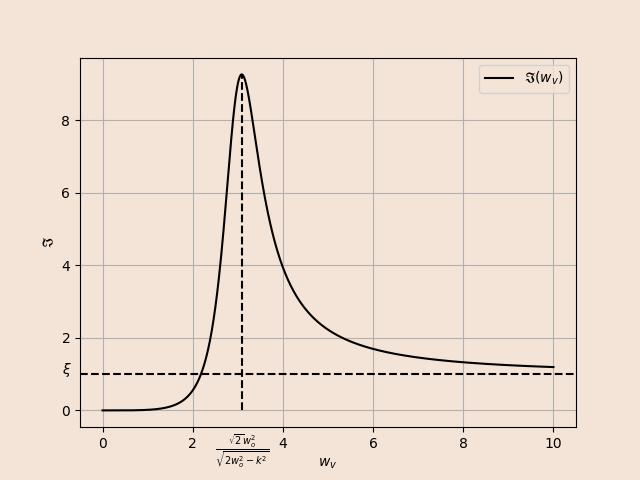
\includegraphics[width=1\textwidth]{sours_img/omega.jpg}
    \caption{Еденицами измерения по оси y выступает $\xi$}
    \label{pict:j_w}
\end{figure}

Как мы видим на графике прослеживается явный максимум в зависимоти $\mathfrak{I}(w_v)$ 
а то значит, что налетающая волнап попала в резоннас с диполем. 

\begin{figure}[H]
    \centering
    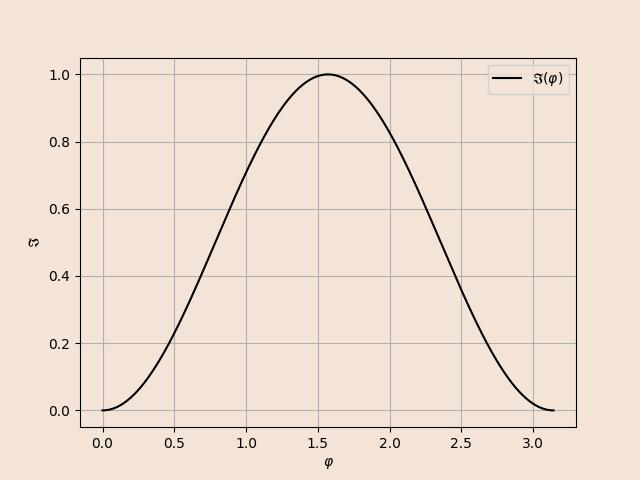
\includegraphics[trim={0 0 0 0},clip,width=1\textwidth]{sours_img/phi.jpg}
    
    \label{pict:J_phi}
\end{figure}


